Previous chapters introduced several algorithms for robot localization and state estimation that are based on a probabilistic framework. In particular, the Bayes filter was first introduced as a fundamental approach to the problem, which uses a probabilistic state transition model and a measurement model to recursively update a belief distribution over possible states. A set tractable implementations of the Bayes filter that model the belief distribution in a \textit{parametric} way, for example using Gaussian distributions, was then presented (in particular the Kalman and extended Kalman filters).
These filters leverage the structure of the parametric belief distribution to provide a computationally efficient approach to dealing with continuous state spaces (which have an infinite number of states). For example the Gaussian distribution represents a continuous distribution through a \textit{finite} set of parameters: the mean and covariance.
However there are also other implementations of Bayes filter that can be efficiently used in continuous state spaces that are \textit{non-parametric}. 

\notessection{Nonparametric Filters}
\cite{ThrunBurgardEtAl2005}
In contrast to parametric filters, \textit{non-parametric} filters do not make assumptions on the structure of the belief distribution. This can be a desirable property for applications in robotics where rigid structures in the belief distribution may result in poor performance. A classic example is that the Gaussian distributions used in the Kalman filter and EKF are unimodal, which cannot express the possibility that two distinct ``high probability'' states might exist at the same time.
Non-parametric filters on the other hand generally represent the belief distribution in an unstructured way, for example through a finite number of samples drawn from the distribution, which allows for more expressive distributions.
This chapter introduces two main approaches for non-parametric filtering: the \textit{histogram filter} and the \textit{particle filter}.

\subsection{Histogram Filter}
The histogram filter is essentially a modification of the discrete Bayes filter presented earlier to work in continuous state spaces. In particular, the continuous state space is decomposed into a finite number of regions and the belief is represented over the discretized space by collecting the finite number of probabilities of the state being in each discretized region.

In particular for the random state variable $X_t$, the continuous state space $\text{dom}(X_t)$ is decomposed into a finite set of regions (often called \textit{bins} in the context of histogram filters):
\begin{equation}
\text{dom}(X_t) = \x_{1,t} \cup \x_{2,t} \cup ... \cup \x_{K,t},
\end{equation}
where $\x_{k,t}$ is the $k$-th ``bin''.
For example, if the one-dimensional random variable $X$ could take on values in the interval $[a,b]$ then one possible decomposition would be to split the interval into a finite number of sub-intervals with equal width.
The belief distribution is then defined in non-parametric way by simply specifying a probability $p_{k,t}$ to each bin $\x_{k,t}$. A probability density function can then be defined in a piecewise manner:
\begin{equation}
p(\x_t) = \frac{p_{k,t}}{\lvert \x_{k,t} \rvert}, \quad \x_t \in \x_{k,t},
\end{equation}
where $\lvert \x_{k,t} \rvert$ denotes the ``area'' or ``volume'' of the bin.
This definition implies that the probability that the random variable $X_t$ takes on \textit{any} value in the bin $\x_{k,t}$ is equal to $p_{k,t}$.

The prediction and measurement update steps of the Bayes filter are then accomplished by also discretizing the state transition and measurement models by computing a representative ``mean'' state for each bin:
\begin{equation}
\hat{\x}_{k,t} = \lvert \x_{k,t} \rvert ^{-1}\int_{\x_{k,t}}x_t d \x_t.
\end{equation}
The state transition model $p(\x_{k,t} \mid \bu_t, \x_{i,t-1})$ that defines the probability of transitioning from one bin to another is then approximated in terms of the mean bin states by:
\begin{equation}
p(\x_{k,t} \mid \bu_t, \x_{i,t-1}) \approx \eta \lvert \x_{k,t} \rvert p(\hat{\x}_{k,t} \mid \bu_t, \hat{\x}_{i,t-1}),
\end{equation}
where $p(\hat{\x}_{k,t} \mid u_t, \hat{\x}_{i,t-1})$ is the original (non-discretized) state transition model evaluated at the mean bin states $\hat{\x}$ and $\eta$ is a normalization constant\footnote{In the case that the bin areas $\lvert \x_{k,t} \rvert$ are equal, these terms can be absorbed into the normalization constant.}.

The discretization of the measurement model is accomplished in a similar manner, with the discretized model given by:
\begin{equation}
p(\z_t \mid \x_{k,t}) \approx p(\z_t \mid \hat{\x}_{k,t}).
\end{equation}
In other words, the measurement probability associated with a bin is approximated by the measurement probability associated with the mean bin state $\hat{\x}_{k,t}$.

After the discretization has been performed, the discrete Bayes filter algorithm from before can be directly applied by iterating over each bin and updating the probability $p_{k,t}$.

\subsection{Particle Filter}
The particle filter is another non-parametric filter that provides a computationally tractable implementation of the Bayes filter for continuous state spaces. This filter represents the belief distribution by a finite set of random samples called particles, which are denoted by:
\begin{equation}
\mathcal{X}_t \coloneqq \{\x_t^{[1]}, \x_t^{[2]},..., \x_t^{[M]}\}.
\end{equation}
Each particle $\x_t^{[m]}$ represents a hypothesis about the true state $\x_t$, and therefore regions of the state space with more particles correspond to regions of high probability.
Ideally, the particles are distributed according to the current belief:
\begin{equation}
    \x_t^{[m]} \sim p(\x_t \mid \z_{1:t}, \bu_{1:t}) = bel(\x_t),
    \label{bel-posterior}
\end{equation}
but theoretically this only occurs as $M\rightarrow \infty$. Instead the set of particles approximately represents the belief distribution, and in practice around $M\approx 1000$ samples tends to be sufficient (but of course this depends on the application).

The particle filter updates the belief (via a prediction and measurement correction step) by manipulating the prior set of particles $\mathcal{X}_{t-1}$ to yield a new set of particles $\mathcal{X}_t$. The prediction step is implemented by considering each particle $\x_{t-1}^{[m]}$ in the prior set $\mathcal{X}_{t-1}$ and sampling from the state transition model a new ``predicted'' sample $\bar{\x}_{t}^{[m]} \sim p(\x_t \mid \bu_t, \x_{t-1}^{[m]})$. An importance factor $w_{t}^{[m]}$ is then defined for the predicted sample $\bar{\x}_{t}^{[m]}$ based on how well the observed measurement matches the prediction. Specifically, the importance factor is computed as $w_t^{[m]} = p(\z_t \mid \bar{\x}_t^{[m]})$. The predicted particles $\bar{\x}_{t}^{[m]}$ and their associated weights $w_t^{[m]}$ can then be collected in a new particle set $\bar{\mathcal{X}}_t$, which represents the predicted belief distribution $\overline{bel}(\x_t)$.
The correction step is then accomplished by simply resampling (with replacement) a new set of $M$ particles from the predicted set $\bar{\mathcal{X}}_t$ with a probability proportional to the weights $w_t^{[m]}$. This procedure performs the measurement correction by giving preference in the new sample set to those predicted particles that showed higher correlation to the measurement $\z_t$.
The resampled points are then collected in a new set $\mathcal{X}_t$ that defines the posterior belief distribution.
This algorithm is also outlined in Algorithm \ref{alg:particle} and a few iterations of the algorithm for a simple robot localization problem are shown in Figure \ref{fig:Particle_filter}.

\begin{algorithm}[ht]
 \KwData{$\mathcal{X}_{t-1}, \bu_{t}, \z_{t}$}
 \KwResult{$\mathcal{X}_{t}$}
 $\bar{\mathcal{X}}_{t} = \mathcal{X}_t = \emptyset$\\
 \For{$m=1$ \KwTo $M$}{
  Sample $\bar{\x}_{t}^{[m]} \sim p(\x_t\mid \bu_t, \x_{t-1}^{[m]})$\\
  $w_t^{[m]} = p(\z_t \mid \bar{\x}_{t}^{[m]})$\\
  $\bar{\mathcal{X}}_{t} = \bar{\mathcal{X}}_{t} \cup \big(\bar{\x}_{t}^{[m]}, w_t^{[m]} \big)$\\
 }
 \For{$m=1$ \KwTo $M$}{
  Draw $i$ with probability $\propto w_t^{[i]}$\\
  Add $\bar{\x}_{t}^{[i]}$ to $\mathcal{X}_t$
 }
 \Return $\mathcal{X}_t$
 \caption{Particle Filter Algorithm}
 \label{alg:particle}
\end{algorithm}

Note that the concept of resampling in the correction step can be quite important for reasons beyond just updating the belief for the measurement correction. In particular, without the resampling step over time some of the particles would drift to regions of low probability and there would be fewer particles to represent the regions of high probability. The resampling step can therefore be viewed as a probabilistic implementation of the Darwinian idea of survival of the fittest: it refocuses the particle set to regions in state space with high posterior probability. This helps from a computational efficiency standpoint because it reduces the number of particles that are needed by focusing them on the regions of the state space that matter (i.e. regions of high probability).
\begin{figure}[ht]
\centering
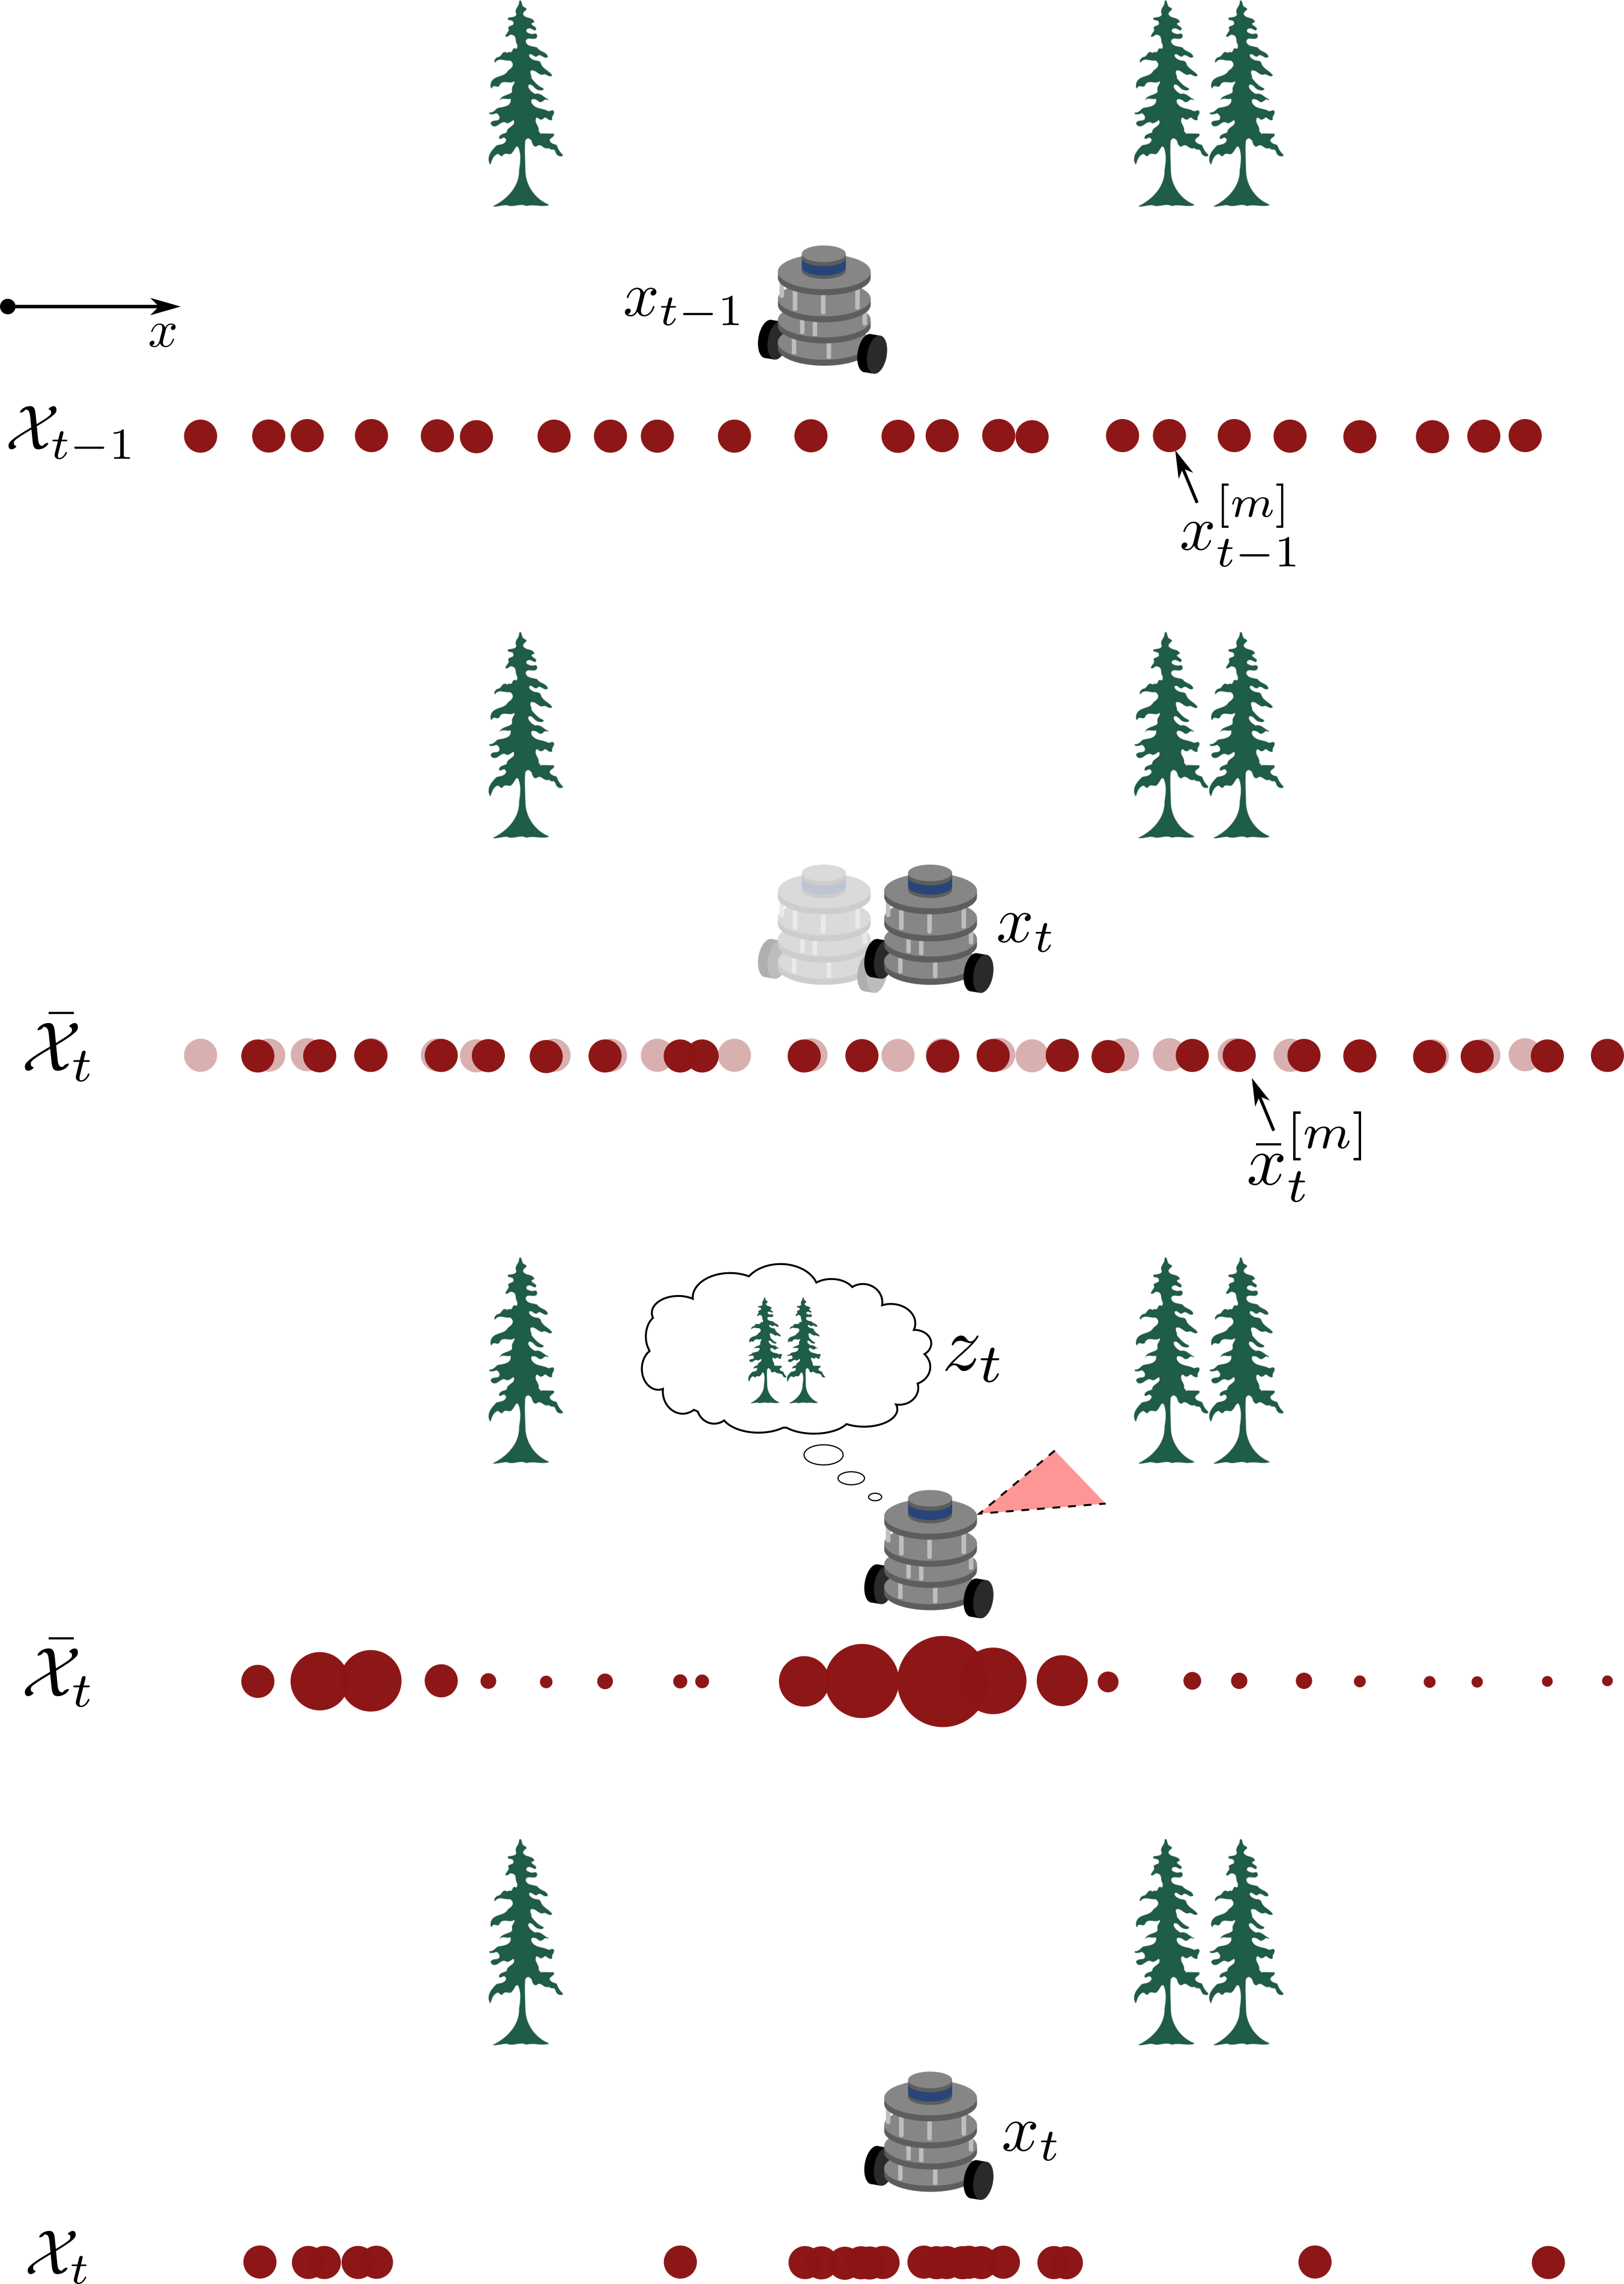
\includegraphics[width=0.8\linewidth]{tex/figs/ch15_figs/particlefilter.png}
\caption{Particle filter used for robot localization. The initial set of particles are first updated according to the transition model, and then weighted according to the observation. Finally, a new set of particles is generated through weighted resampling.}
\label{fig:Particle_filter}
\end{figure}

\subsection{Exercises}
\subsubsection{Monte Carlo Localization}
Complete \textit{Extra Credit: Monte Carlo Localization} located in the online repository:

\vspace{\baselineskip}

\url{https://github.com/PrinciplesofRobotAutonomy/AA274A_HW4},

\vspace{\baselineskip}

where you will implement a particle filter for localizing a robot with line feature extraction, similar to the exercise on EKF localization from the previous chapter.

